\chapter*{About the author}\markboth{About the author}{About the author}

\addcontentsline{toc}{chapter}{About the author}

\begin{wrapfigure}{O}{0.34\textwidth}
%\centering
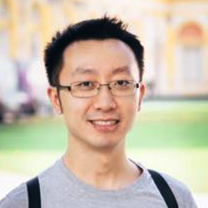
\includegraphics[width=0.34\textwidth, trim=0 0 0 0.8cm]{./0-misc/images/vincent.png}
%\caption{\label{fig:frog2}This is a figure caption.}
\end{wrapfigure}

His research interests include social data analysis, crowd behaviour and crowd management in city events.



\vspace*{\fill}
\pagebreak

\vspace*{0.60cm}
\noindent{\Huge \textbf{Publications}}

\section*{Journal papers}

\begin{enumerate}
%  \item \textbf{Gong, Vincent X.}, et al. "Using social media for attendees density estimation in city-scale events." IEEE Access 6 (2018): 36325-36340.
  \item \textbf{Gong, Vincent X.}, Jie Yang, Winnie Daamen, Alessandro Bozzon, Serge P. Hoogendoorn, and Geert-Jan Houben. "Using social media for attendees density estimation in city-scale events." IEEE Access 6 (2018): 36325-36340.
\end{enumerate}

% to get page numbers a multiple of 8 it may be necessary to add some empty pages

%\pagestyle{plain}\fancyhf{}\markboth{}{}
%\newpage{\mbox{}}

%%% Local Variables: 
%%% mode: latex
%%% TeX-master: "../2007-thesis"
%%% End: 
